% Intrinsic Efficiency
\documentclass[draftcls,onecolumn]{IEEEtran}

%% INCLUDING THE PREAMBLE
%%%%%%%%%%%%%%%%%%%%%%%%%%%%%%%%%%%%%%%%%%%%%%%%%%%%%%%%%%%%%%%%%%%%%%%%%%%
%                                                                         %
%                                 PREAMBLE                                %
%                                                                         %
%%%%%%%%%%%%%%%%%%%%%%%%%%%%%%%%%%%%%%%%%%%%%%%%%%%%%%%%%%%%%%%%%%%%%%%%%%%

%% PACKAGES
\usepackage[]{lineno}
%\linenumbers
\usepackage[usenames,dvipsnames]{xcolor}
\usepackage{microtype}
\usepackage[obeyDraft]{todonotes}
\usepackage{fancyvrb}
\VerbatimFootnotes
\usepackage{algorithmic}

%% GRAPHICS RELATED
\usepackage{graphicx}
\usepackage[outdir=./tmp/]{epstopdf}
\graphicspath{{../images/}{./}{./tmp/}}
\DeclareGraphicsExtensions{.eps, .pdf, .jpeg, .png,}

%% CPATION SETUP
\usepackage{float}
\usepackage{caption}
\usepackage{subcaption}
\captionsetup{belowskip=12pt,aboveskip=4pt}


%% BIBLIOGRAPHY
\bibliographystyle{ieeetr}

%% UNITS
\usepackage{siunitx}

%% EQUATIONS
\usepackage{amsmath}
%\numberwithin{equation}{section}

%% HYPERLINKS
\usepackage[debug]{hyperref}

%%%%%%%%%%%%%%%%%%%%%%%%%%%%%%%%%%%%%%%%%%%%%%%%%%%%%%%%%%%%%%%%%%%%%%%%%%%
%                                                                         %
%                             Listing Setup                               %
%                                                                         %
%%%%%%%%%%%%%%%%%%%%%%%%%%%%%%%%%%%%%%%%%%%%%%%%%%%%%%%%%%%%%%%%%%%%%%%%%%%
\usepackage{listings}
\lstset{ %
    language=C++,
    basicstyle=\footnotesize\ttfamily,
    numbers=left,
    numberstyle=\tiny\color{gray},
    stepnumber=2,
    numbersep=5pt,
    backgroundcolor=\color{white},
    showspaces=false,
    showstringspaces=false,
    showtabs=false,
    frame=single,
    rulecolor=\color{black},
    tabsize=2,
    breaklines=true,
    breakatwhitespace=false,
    title=\lstname,
    keywordstyle=\color{blue},
    commentstyle=\color{OliveGreen},
    stringstyle=\color{orange}
}
\DeclareCaptionFont{white}{\color{white}}
\DeclareCaptionFormat{listing}{\colorbox[cmyk]{0.43, 0.35, 0.35, 0.01}{\parbox{\dimexpr\textwidth-2\fboxsep\relax}{#1#2#3}}}
\captionsetup[lstlisting]{format=listing,labelfont=white,textfont=white,singlelinecheck=false,margin=0pt,font={bf,footnotesize}}
%\lstnewenvironment{code}[1][]%
%{ \noindent\minipage{\linewidth}
%	\lstset{#1}
%}
%{\endminipage}
%% USER COMMANDS
\usepackage{isotope}
\newcommand{\iso}{\isotope}
\newcommand{\figurewidth}{\textwidth}
\newcommand{\micron}{$\mu$m}


% index generation
\usepackage{makeidx}
\usepackage{exercise}
\makeindex
 
% 'list of notations' generation
\usepackage[refpage]{nomencl}  % refer to the page where notation appears
\newcommand{\definevar}[2]{#1 #2\nomenclature{#1}{#2}}
\renewcommand{\nomname}{List of Notations}
\renewcommand*{\pagedeclaration}[1]{\unskip\dotfill\hyperpage{#1}}
\makenomenclature
 


%% Start of the document
\begin{document}
\title{Intrinsic Efficiency Calculations}
\author{Matthew J. Urffer}
\date{\today}
\maketitle

% Nomenclature
\printnomenclature
\printindex

% Tables of Contents, Figures, Tables
\listoftodos
\tableofcontents
\listoffigures
\listoftables
\lstlistoflistings
\section{Intrinsic Efficiency}
The intrinsic efficiency is defined as \eqref{eqn:intEffDef} \cite{knoll_radiation_2009}.
\begin{align}
  \label{eqn:intEffDef}
  \epsilon_{int} = \frac{N_c}{N_i}
\end{align}
where:
\begin{itemize}
  \item[] \definevar{$\epsilon_{int}$}{intrinsic efficiency},
  \item[] \definevar{$N_c$}{number of counts recorded by the detector}, and
  \item[] \definevar{$N_i$}{quanta of radiation incident upon the detector}.
\end{itemize}
The quanta of radiation incident upon the detector can be subdivided into two components: the source strength and the solid angle.
The composition of $N_i$ is shown in \eqref{eqn:QuantaIncidentDef}
\begin{align}
  \label{eqn:QuantaIncidentDef}
  N_i = \Omega S_0
\end{align}
where:
\begin{itemize}
  \item[] \definevar{$S$}{source strength}, and 
  \item[] \definevar{$\Omega$}{solid angle}.
\end{itemize}
In general the source strength according the half-life of the source \eqref{eqn:HalfLife}, where \definevar{$S_0$}{initial source strength}, \definevar{$t_{1/2}$}{half life} and \definevar{$t$}{age of source}.
\begin{align}
  \label{eqn:HalfLife}
  S = S_0 e^{-\frac{\ln{2}}{t_{1/2}} t}
\end{align}

The solid angle factor is computed using MCNPX. 
A F1 tally is used over the detector surface with two cosine bins, $-1<\cos\theta<0$ and $0<\cos\theta<1$.
As macro-bodies are used for the surfaces of the detector, $-1<\cos\theta<0$ represents the particles that cross into the surface and $0<\cos\theta<1$ the particles that leave the surface.
The MCNPX simulation was benched marked against GS20 and against polymer films.
Tables are provided for common geometries; other geometries can be found by interpolation.

It is often desirable to express the intrinsic efficiency for a given channel number or Mathematical Lower Level Discriminator (MLLD)\footnote{The MLLD behaves essentially as a physical lower level discriminator in that all counts below this value are discarded}.
The intrinsic efficiency can then be expressed as a function of this MLLD \eqref{eqn:MLLDDef}.
The number of counts recorded by the detector can be expressed as the integral of \definevar{$p(x)$}{spectra function} from some lower bound (the MLLD) to an upper bound, the end of the spectra.
\begin{align}
	\label{eqn:MLLDDef}
	\epsilon_{int} &= \frac{\int_{MLLD}^\infty p(x)dx}{N_i}
\end{align}

\subsection{Neutron Intrinsic Efficiency}
The number of counts upon a detector is measured using the neutron irridiator facility.
The quanta of radiation incident upon the detector is found from MCNPX calculations.
This consists of two parts: 1) determining the number of neutrons crossing the detector surface in the lead and cadmium wells and, 2) determining the source strength.

The \iso[252]{Cf} source was \SI{0.59}{\ug} on July 2, 2009.
Given that the half-life of \iso[252]{Cf} is 2.65 years and \iso[252]{Cf} has a spontaneous neutron emission rate of \SI{2.3E6}{neutron\per\second\per\micro\gram} the source strength at any given time can be calculated as \eqref{eqn:Cf252SourceStrength}.
\begin{align}
  \label{eqn:Cf252SourceStrength}
  S &= S_0 e^{-\frac{\ln{2}}{t_{1/2}} t} \\ \notag 
    &= \SI{0.59}{\ug} \iso[252]{Cf} \;\frac{\SI{2.3E6}{neutron\per\second}}{\si{\ug} \iso[252]{Cf}}\; e^{-\frac{ \ln{2}}{\SI{2.54}{year}}t}  \\ \notag
    &= \SI{1.357E6}{neutron\per\second}\; e^{-\frac{ \ln{2}}{\SI{2.54}{year}}t} 
\end{align}

Table \ref{tab:NeutronSolidAngle} summarizes the incident flux for a number of different detector sizes and heights.

\begin{table}
	\centering
	\caption{Simulated Neutron Solid Angle for Various Film Radii}
	\label{tab:NeutronSolidAngle}
	\begin{tabular}{c | c c}
 		Thickness & \SI{1}{\cm} & \SI{1.27}{\cm}  \\ \hline
		0.5 & \num{8.03E-4} & \\
		0.2 & \num{6.34E-4} & \num{9.87E-4} \\
		0.1 & \num{5.77E-4} & \num{9.31E-4} \\ 
	\end{tabular}
\end{table}

It should be noted that there is considerable variation in the neutron flux in the detector wells, as shown in \ref{fig:NeutronFluxProfiles}.
Thus, even though the calculations are accurate to less than a present, the real error on the intrinsic efficiency will be much higher due to uncertainty in where the detector was placed in the well.
\begin{figure}
	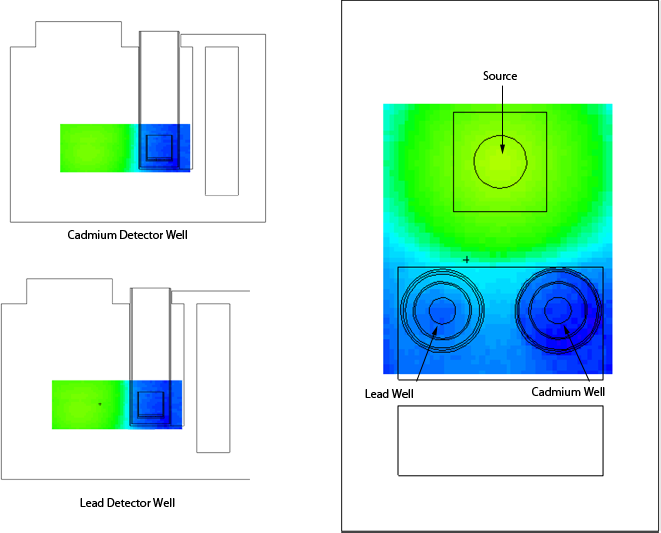
\includegraphics[width=\textwidth]{SpatialNeutronFlux}
  \caption{Neutron Flux Profiles of the Lead and Cadmium Wells}
  \label{fig:NeutronFluxProfiles}
\end{figure}

\subsection{Gamma Intrinsic Efficiency}
The gamma intrinsic efficiency is calculated by a combination of simulation to determine the solid angle that the detector subtends and radioactive decay.
The gamma irridiator consists of a \SI{97}{\micro Ci} \iso[60]{Co} (January 1st, 2012).
The incident flux is calculated according to \eqref{eqn:Co60SourceStrength}, and the solid angle is tabulated in Table \ref{tab:GammaSolidAngle}.
\begin{align}
  \label{eqn:Co60SourceStrength}
  S &= S_0 e^{-\frac{\ln{2}}{t_{1/2}} t} \\ \notag 
    &= \SI{97}{\micro Ci} \iso[60]{Co}\; \frac{\SI{1.3E10}{decay\per\second}}{\si{Ci}} \;\frac{2\text{photon}}{decay}\;e^{-\frac{ \ln{2}}{\SI{5.27}{year}}t}  \\ \notag
    &= \SI{7.178E6}{photon\per\second}\;e^{-\frac{ \ln{2}}{\SI{5.27}{year}}t} 
\end{align}
\begin{table}
	\centering
	\caption{Simulated Gamma Solid Angle for Various Film Radii}
	\label{tab:GammaSolidAngle}
	\begin{tabular}{c | c c c c c c}
Thickness (\si{\cm})	&	\SI{1}{\cm}	&	\SI{1.27}{\cm}	&	\SI{1.905}{\cm}	&	\SI{2}{\cm}	&	\SI{2.5}{\cm}	&	\SI{2.54}{\cm} \\ \hline
0.0025	&	0.0060	&	0.0095	&	0.0206	&	0.0226	&	0.0347	&	0.0357\\
0.005	&	0.0060	&	0.0095	&	0.0206	&	0.0226	&	0.0347	&	0.0357\\
0.01	&	0.0060	&	0.0095	&	0.0206	&	0.0226	&	0.0347	&	0.0357\\
0.015	&	0.0060	&	0.0095	&	0.0206	&	0.0226	&	0.0347	&	0.0357\\
0.03	&	0.0060	&	0.0095	&	0.0206	&	0.0227	&	0.0347	&	0.0357\\
0.1	&	0.0060	&	0.0096	&	0.0207	&	0.0227	&	0.0348	&	0.0358\\
0.2	&	0.0061	&	0.0097	&	0.0209	&	0.0229	&	0.0349	&	0.0360\\
0.5	&	0.0063	&	0.0099	&	0.0212	&	0.0232	&	0.0353	&	0.0364\\
1	&	0.0066	&	0.0103	&	0.0217	&	0.0237	&	0.0359	&	0.0379\\
2	&	0.0071	&	0.0109	&	0.0225	&	0.0247	&	0.0371	&	0.0382\\
3	&	0.0075	&	0.0114	&	0.0233	&	0.0255	&	0.0381	&	0.0392\\
4	&	0.0079	&	0.0119	&	0.0240	&	0.0262	&	0.0390	&	0.0401\\
	\end{tabular}
\end{table}
\todo[inline]{There seems to be something funky with the 2.54 cm runs.  Same input deck / script, but somehow the fluence decreases with the film thickness, and this isn't observed with the 2.5 cm runs.  I don't get any warnings about a particle lost (with a run of 1 million) so something really funky is going on. It is definitely a funky geometry thing since if I make the it a tiny bit smaller}
The gamma irridiator detector well is encased in a 1/2 inch steel pipe which is surrounded by lead, providing a beam like geometry while also introducing lower energy photons. 
The contribution of these lower energy photons is shown if Figure \ref{fig:PhotonFluxAllEnergies}.
\begin{figure}
  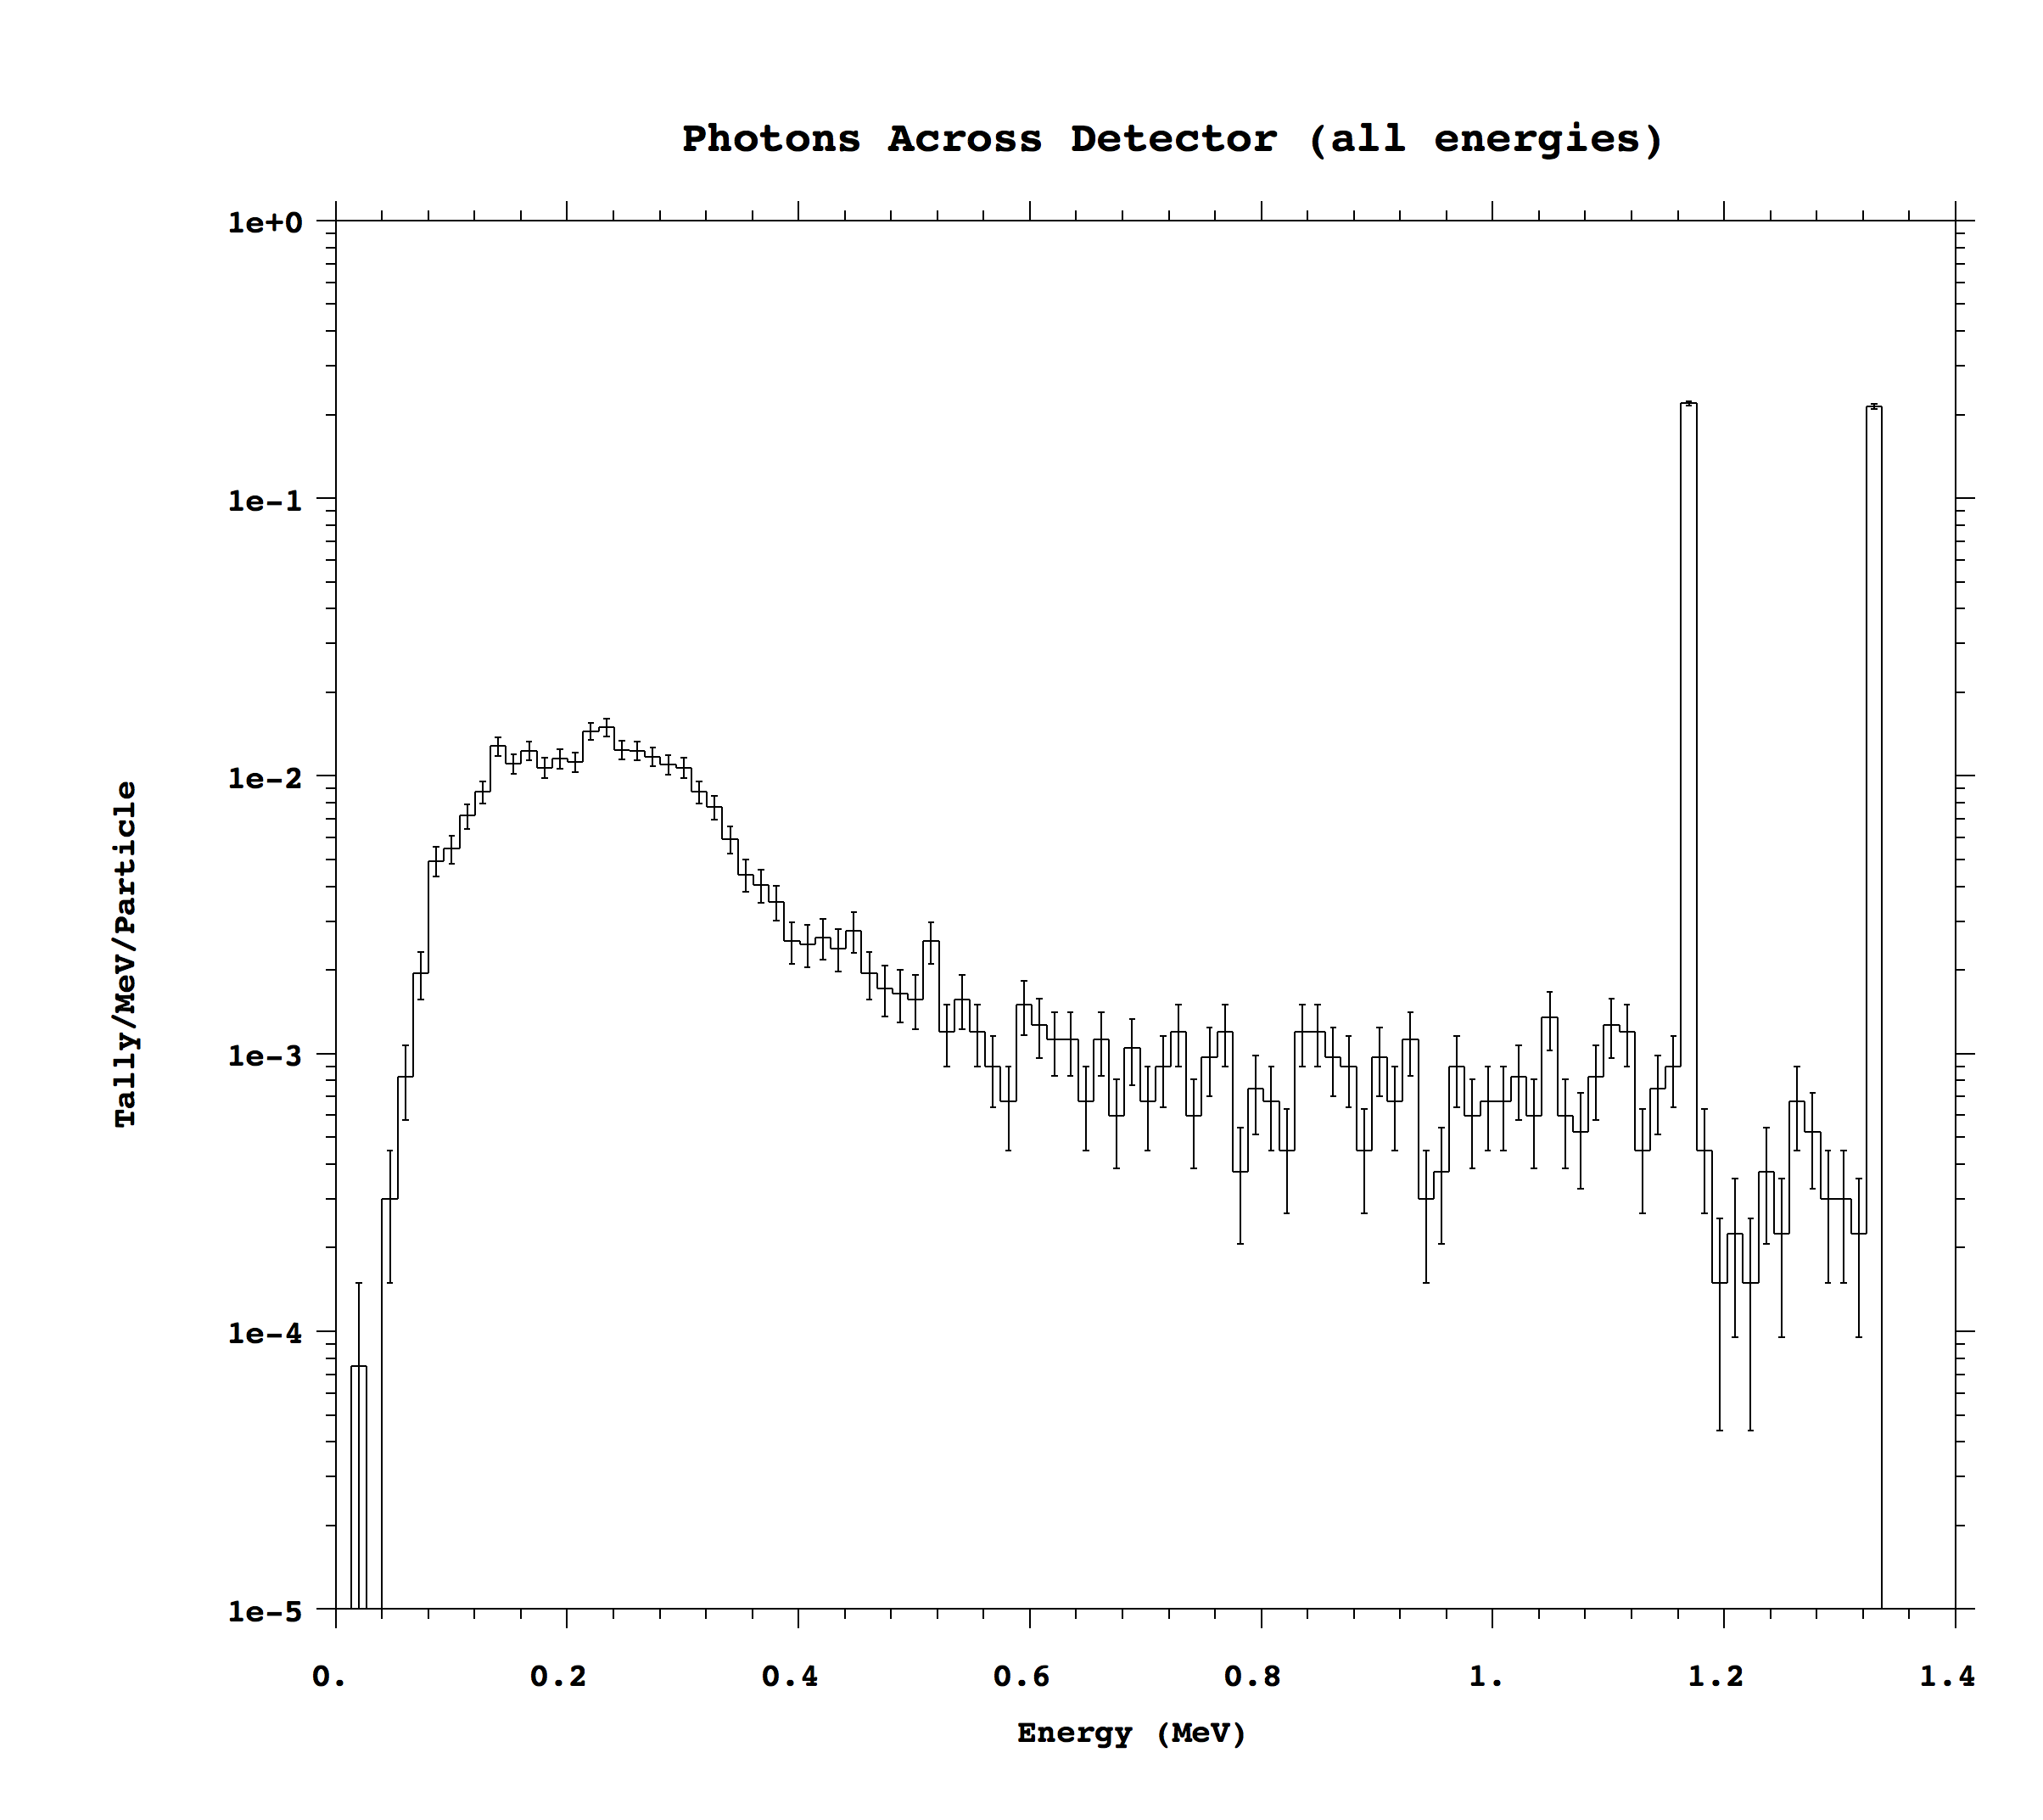
\includegraphics[width=\textwidth]{PhotonEnergyDist}
	\caption{Photon Flux into Detector}
  \label{fig:PhotonFluxAllEnergies}
\end{figure}
Table \ref{tab:GammaSolidAngle} considers the contributions from all sides, but it is evident that the contributions from the side scattering is not large as 100 times increase in the thickness (\SI{50}{\um} to \SI{5}{\mm}) results in only a 4\% increase in the number of particles crossing the detector.

\pagebreak
\subsection{Examples}
\begin{Exercise*}[label={LiBorateGlass},title={Li borate glass},name={Example}]
A sample measured on April 4, 2013 \SI{1.327}{\g} sample of $\iso[6]{Li}\text{B}_4\text{O}_7$ glass was fabricated by John Auxier.
This sample was roughly rectangular in shape (\SI{1.3}{\cm} by \SI{2.2}{\cm}) with a thickness of \SI{2.7}{\mm}.
The sample was measured April 4, 2013.



The neutron intrinsic efficiency is calculated according to \eqref{eqn:intEffDef} with the source strength as supplied in \eqref{eqn:Cf252SourceStrength}, with the source aging $t = 3.76 \text{yr}$ to the measurement.
\begin{align}
    S &= \SI{1.357E6}{neutron\per\second} e^{-\frac{ \ln{2}}{\SI{2.54}{year}}\SI{3.76}{year}} \\ \notag
      &= \SI{4.86E5}{neutron\per\second}
\end{align}
Approximating the sample as a cylinder (maintaining the area of the faces) yields a radius of \SI{0.95}{\cm}.
\begin{align}
	r &= \sqrt{\frac{\SI{1.3}{\cm} \times \SI{2.2}{\cm}}{\pi}} \\ \notag
	& = \SI{0.95}{\cm}
\end{align}
From Table \ref{tab:NeutronSolidAngle} the closest radius is \SI{1}{\cm}.
Linear interpolation is used to calculate the expected solid angle at a thickness of \SI{0.27}{\cm}, and then a ratio of the areas is used to calculate the solid angle at a radius of \SI{0.95}{\cm}.
\begin{align*}
	\frac{A_1}{A_2} &= \frac{\Omega_1}{\Omega_2} \\ \notag
	\Omega_2 &= \frac{r_2^2 \Omega_2}{r_1^2} \\
	 &= \frac{\SI{0.95}{\cm}^2 \num{6.73E-4}}{\SI{1}{\cm}^2}
	 &= \num{6.07E-4}
\end{align*}
This is then multiplied by the source strength on the date of the measurement, \SI{4.86E5}{neutron\per\second}, to determine the flux.
\begin{align*}
 	N_i &= \Omega S \\
	 &= \num{6.07E-4} \; \SI{4.86E5}{neutron\per\second} \\
   &= \SI{284}{neutron\per\second}
\end{align*}

The \iso[60]{Co} source has aged 459 days (1.26 years) since the measurement.
The source strength is then:
\begin{align}
  S &= \SI{7.178E6}{photon\per\second}\;e^{-\frac{ \ln{2}}{\SI{5.27}{year}}\SI{1.26}{year}} \\ \notag
    &= \SI{6.08E6}{photon\per\second}
\end{align}
Once again interpolation is used to calculated the solid angle.
\begin{align*}
	\frac{A_1}{A_2} &= \frac{\Omega_1}{\Omega_2} \\ \notag
	\Omega_2 &= \frac{r_2^2 \Omega_2}{r_1^2} \\
	 &= \frac{\SI{0.95}{\cm}^2 \num{6.17E-3}}{\SI{1}{\cm}^2}
	 &= \num{5.57E-3}
\end{align*}
This is then multiplied by the source strength on the date of the measurement, \SI{6.08E6}{photon\per\second}, to determine the flux.
\begin{align*}
 	N_i &= \Omega S \\
	 &= \num{5.57E-3} \; \SI{6.08E6}{photon\per\second} \\
      &= \SI{33.9E4}{neutron\per\second}
\end{align*}
It is then possible to plot the intrinsic efficiency in your favorite computational package.

\end{Exercise*}
\begin{Exercise*}[label={LiquidSample},title={Liquid Sample},name={Example}]
The neutron fluence over a \SI{5}{\milli\liter} vial is desired in order to compute the intrisinic efficiency of neutron samples fabricated and measured by members of SCSU.
MCNPX calculations for the solid angle, $\Omega$ show that \SI{4.477E=3}{neuron\per source particle} cross the sample in the lead well, and \SI{1.475E-3}{neuton\per source particle} cross the sample in the cadium well.
Thus the net particles crossing the detector is $\Omega_{\text{net}} =\SI{4.477E=3}{neuron\per source particle} - \SI{1.475E-3}{neuton\per source particle} =\SI{3.002E-3}{neuton\per source particle} $.
Depending on when the sample was measured the number of neutrons crossing the sample can be calculated by multipy \eqref{eqn:Cf252SourceStrength} by the solid angle calculated above.

The SCSU samples where not measured in the \iso[60]{Co} irridiator but rather by placing a source on the outside of the sample.

\end{Exercise*}

% Bibliography
\bibliography{../Zotero}

\section{Appendix}
The generated MCNPX tables was based upon a script input deck for gamma and neutrons in \verb+MCNP/IncidentFlux+.
An analysis script was written in python in order to extract the necessary lines from the output decks.
\end{document}

